\documentclass[10pt,conference,final]{IEEEtran}
\usepackage[top=1.5cm, bottom=1.5cm, left=1.5cm, right=1.5cm]{geometry}

\usepackage[british]{babel}
\usepackage[hyphens]{url}
\usepackage{paralist}
\usepackage{graphicx}
\usepackage[noadjust]{cite}
\usepackage[pdftex,colorlinks=true]{hyperref}

\IEEEoverridecommandlockouts

\begin{document}
\bstctlcite{IEEEexample:BSTcontrol}

% title
\title{``Can I Implement Your Algorithm?'':\\ A Model for Reproducible Research Software}

% author names and affiliations
% use a multiple column layout for up to three different
% affiliations
\author{\IEEEauthorblockN{Tom Crick\thanks{Tom Crick would like to
      acknowledge financial support from the Software Sustainability
      Institute as a 2014 Fellow.}}
\IEEEauthorblockA{Department of Computing\\
Cardiff Metropolitan University\\
Cardiff, UK\\
Email: {\url{tcrick@cardiffmet.ac.uk}}}
\and
\IEEEauthorblockN{Benjamin A. Hall and Samin Ishtiaq}
\IEEEauthorblockA{Microsoft Research\\
Cambridge, UK\\
Email: {\url{{benhall,samin.ishtiaq}@microsoft.com}}}}

\maketitle

\begin{abstract}
The reproduction and replication of novel scientific results has
become a major issue for a number of disciplines. In computer science
and related disciplines such as systems biology, the issues closely
revolve around the ability to implement novel algorithms and
approaches. Taking an approach from the literature and applying it in
a new codebase frequently requires local knowledge missing from the
published manuscripts and project websites. Alongside this issue,
benchmarking, and the development of fair, and widely available
benchmark sets present another barrier. In this paper, we outline
several suggestions to address these issues, driven by specific
examples from a range of scientific domains.  Finally, based on these
suggestions, we propose a new open platform for scientific software
development which effectively isolates specific dependencies from the
individual researcher and their workstation and allows faster, more
powerful sharing of the results of scientific software engineering.
\end{abstract}

\IEEEpeerreviewmaketitle

\section{Introduction}

Marc Andreessen famously said in 2011 that ``{\emph{software is eating the
world}}''~\cite{andreessen:2011}. It is true: we clearly live in a
computational world, with our everyday communications, entertainment,
shopping, security, transportation, \dots\ all heavily dependent on
(or replaced by) software.

This is particularly true for science and engineering. A 2012 report
by the Royal Society stated that computational techniques have
``{\emph{moved on from assisting scientists in doing science, to
transforming both how science is done and what science is
done}}''~\cite{rssaaoe:2012}. New experiments, simulations, models,
benchmarks, even proofs cannot be done without software. And this
software does not consist of simple hack-together, use-once,
throw-away scripts; scientific software repositories contain
thousands, perhaps millions, of lines of code and they need to be
actively supported and maintained. More importantly, with
reproducibility being a fundamental tenet of science, they need to be
re-useable.

However, if we want to be truthful about this, then the scientific
literature related to software tools often do not appear to be
adhering to the rules themselves~\cite{nature:2011}. How many of them
are reproducible? How many explain their experimental methodologies,
in particular the basis for their benchmarking? In particular, can we
build the code~\cite{collberg-et-al:2014}? We, the authors, are
perhaps as guilty as anyone in the past, where we have succumbed to
publishing papers~\cite{crick-et-al:2009,Berdine2011SLAyer} with
benchmarks and promises of code to be released in the near future.

There are many reasons why the wider scientific community is in this
state. We are experiencing significant changes in academic
dissemination and publication, especially the open access movement,
with new models being
proposed~\cite{stodden-et-al:2013,fursin+dubach:2014}.  There are
numerous non-technical impediments to making software maintainable and
re-useable, too. The pressure to ``make the discovery'' and publish
quickly disincentivises careful software development. Releasing code
prematurely is often seen to give your competitors an advantage, but
we should be shining light into these ``black
boxes''~\cite{morin-et-al:2012}. In essence: better software, better
research~\cite{goble:2014}.

Things can and should be much better. In this paper, we present a call
to action with a set of recommendations which we hope will lead to
better, more sustainable, more re-useable software, to move towards an
imagined future practice of software development and usage in science
and engineering.  The basis for many of these recommendations is the
basic scientific tenet of openness. There has been previous work in
this area~\cite{sim-et-al:2003,chirigati-et-al:2013}, as well as a
range of manifestos for reproducible research and community
initiatives, such as cTuning\footnote{\url{http://ctuning.org/}} and
the Recomputation
Manifesto~\cite{gent:2013}\footnote{\url{http://www.recomputation.org/}},
along with curated recommendations on where to publish research
software\footnote{\url{http://www.software.ac.uk/resources/guides/which-journals-should-i-publish-my-software}}.

\section{Can I implement your algorithm?}

Reproducibility is a basic tenet of good science. Yet many
descriptions of algorithms are too high-level, too obscure, too
hand-wavey to allow an easy implementation by a third party. A line in
the algorithm might say: ``We pick an element from the frontier set''
but which element do you pick? Will the first one do? Why will any
element suffice? Sometimes the author would like to give more
implementation detail but is constrained by the paper page
limit. Sometimes the authors' description in-lines other algorithms or
data structures that perhaps only that author is familiar with.

We recommend here that a paper must describe the algorithm in such a
way that it is implementable by any reader of that algorithm. This is
subjective, of course. So, we also recommend that good scientific
conferences have a special track for papers that only re-implement
past papers' algorithms, techniques, or tools.


\section{Set the code free} 

There can be no better proof that your algorithm works, than if you
provide the source code of an implementation. Software development is
hard, but sharing and using others code is relatively easy.

% how long? change link to ref?
A long time ago, Richard Stallman (founder of the GNU Project and Free
Software Foundation) postulated that all code would be
free\footnote{\url{http://www.gnu.org/philosophy/shouldbefree.html}}
and we would make our money by consulting on the code.  Somewhat
ironically, this is the case for a significant part of the computing
industry now. There are, of course, hard commercial pressures for
keeping code closed-source. Even in the scientific domain, scientists
and their collaborators may wish to hold onto their code as a
competitive advantage, especially if there exists larger competitors
who could use the available code to ``reverse scoop'' the inventors,
charging into a promising new research area opened by the inventors.

Closed source is one thing. Licenses that deny the user from viewing,
modifying, or sharing the source are another thing. There are, however, even
licences on widely adopted tools like GAUSSIAN~\cite{Giles2004} that
prohibit even analysing software performance and behaviour.
 
There is little doubt that, if science wants to be open and free, then
the code that underlies it too needs to be open and free. Code that is
available for browsing, modifying, and forking facilitates testing and
comparison, and promotes competition. We recommend that code be
published under an appropriate open source license~\cite{osl}; while
we defer legal discussion of any particular licences, BSD and Apache
are good, flexible ones.
% IANAL...

A wide variety of licenses exist for molecular dynamics software, with
different degrees of openness (GROMACS is LGPL~\cite{Hess2008},
CHARMM and Desmond are Academic/Commercial software
licences~\cite{Brooks2009,Bowers2006}, Amber and NAMD are custom
open-like licences). Z3 is an example from the verification area: the
code itself is not open source, but the MSR-LA that allows the source
code to be read, copied, forked for academic use, provides researchers
in the field much more than before~\cite{deMoura2012Z3open}.

Ultimately: set the code free. Put it on a public space such as GitHub, where it
is easy to share and fork. You should embrace the spirit of the CRAPL
academic-strength open source
license\footnote{\url{http://matt.might.net/articles/crapl/}} and
publish your code -- it is good enough~\cite{barnes:2010}.


\section{Be a better person}

If you have the skills and the experience, you can create better
software. We have seen the emergence of initiatives, such as the Software
Carpentry\footnote{\url{http://software-carpentry.org/}}, Software
Sustainability Institute\footnote{\url{http://www.software.ac.uk/}}
and the UK Community of Research Software
Engineers\footnote{\url{http://www.rse.ac.uk}} to cultivate
world-class research through software, develop software skills and
raise the profile of research software engineers.

Some scientists may not have had any formal, or even informal,
training in programming. Even basic training in software engineering
concepts like version control, unit testing, etc, can help improve the
quality of the software written
enormously\cite{Wilson2014}\footnote{Also see:
\url{http://philipwfowler.wordpress.com/2013/12/19/the-oxford-software-carpentry-boot-camp-one-year-on/}}.
Interestingly, many of these concepts are taught to computer science
undergraduates, but it could be argued that they are taught at the
wrong time of the engineers' careers, where the importance of complex,
long-running projects is not yet appreciated.

These should be regarded as fundamental literacies for scientists and
engineers: we recommend that basic programming and computational
skills are taught as a core at undergraduate and postgraduate level.


\section{Latin is the language of God} 

There really is no other scientific or technical field where its
participants can just make up a non-principled artefact like a
programming language so easily. In a way, it says how much of a
``commons'' computer science is, that anyone and his dog can create a
new programming language, API, framework or compiler. This clearly has
advantages and disadvantages.

What is clear is that the use of a principled, high-level programming
language to write your software in helps hugely with the
maintainability and robustness of the software produced. Such
programming languages impose constraints like types: that you can
never add a number and a string is the most basic example, but ML's
functors provide principled ways of plugging in components with their
implementations completely hidden. Aggressive type checking avoids a
subset of bugs which can arise due to incorrectly written functions
e.g. well publicised NASA problems with a Mars orbiter\footnote{See:
\url{http://www.cnn.com/TECH/space/9909/30/mars.metric.02/}}.  A
further example is a pressure coupling
bug\footnote{\url{http://redmine.gromacs.org/issues/14}} in
GROMACS~\cite{Hess2008}, which arose due to the inappropriate swapping
of a pressure term with a stress tensor.  A further extension of
types, a concept called units of measure that is implemented in
languages such as F\#, can deal with these kinds of bugs at compile
time. Similarly, problems found using in-house software for
crystallography led to the retraction of five papers~\cite{Miller2006}, due
to a bug which inverted the phases.

High level languages are often more readable than their
competitors. The ``density'' of a program is often seen to be a good
thing, but it is not always the case that a shorter Haskell program is
better to maintain than longer Python/C++ one. Nevertheless, what is
important is the readability of the code itself. A good example here
is from the world of automatic theorem proving: the SSReflect language
is much more readable than the original, standard Coq
language~\cite{GonthierZND13}. SSReflect uses mathematicians'
vernacular for script commands, allows reproducibility of automatic
proof checking because parameters are named rather than numbered. 
Even though these proof scripts are really only ever going to be
run by a machine, they seek to maintain the basic mathematical idea
that a proof should be readable by another mathematician.

\section{Test it to see}

Some models may be chaotic and influenced by floating point errors
(e.g. molecular dynamics), further frustrating testing. For example:
Sidekick is an automated tool for building molecular models and
performing simulations~\cite{Hall2014Sidekick}. Each system is
simulated from an different initial random seed, and under most
circumstances this is the only difference expected between
replicas. However, on a mixed cluster with both AMD and Intel
microprocessors on the nodes, the difference in architecture was found
to alter the number of water molecules added to each system by
one. This meant that the same simulation performed on different
architectures would diverge. Similarly, in a different simulation
engine, different neighbour searching strategies gave divergent
simulations due to the differing order in which forces were summed.

Despite these challenges to testing, unshared code is ultimately
untestable.  Testing new complex scientific software is difficult, as
until the software is complete unit tests may not be available. You
should thus link from shared code -- shared code is more test-able.

\section{Lineage} 

Research software is not just software -- it is the instantiation of
novel algorithms and data structures (or at least novel applications
of data structures). Thus, lineage is important: the code should
include links to papers publishing key algorithms and the
code should include explicit relationships to other projects on the
repository (i.e. {\emph{Project B}} was branched from {\emph{Project
A}}). This ensure that both the researchers and software developers
working upstream of the current project are properly credited,
encouraging future sharing and development. Remember, the people who
did the research are not necessarily the same people as the developers
and maintainers of the software, so it is important to reward both
appropriately with citations (a good way of doing this is the use of
CITATION
files\footnote{\url{http://blog.rtwilson.com/encouraging-citation-of-software-introducing-citation-files/}}).


\section{YMMV}

\begin{figure}[!ht]
\centering
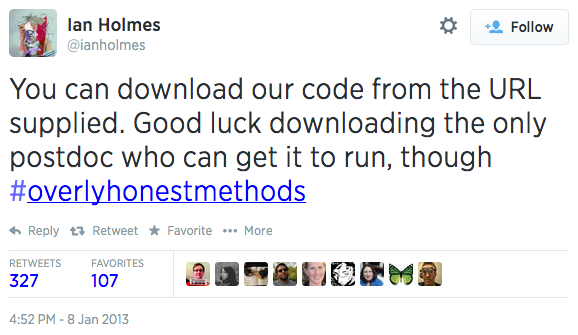
\includegraphics[width=\columnwidth]{overlyhonesttweet.png}
\caption{An \#overlyhonestmethod\newline [source: \url{https://twitter.com/ianholmes/status/288689712636493824}]}
\label{fig:overlyhonestmethod} 
\end{figure}

The tweet is Figure~\ref{fig:overlyhonestmethod} is funny because it
is worryingly true. Often, the tool that the paper describes does not
exist for download. Or runs only on one particular bespoke
platform. Or might run for the author, for a while, but will bit-rot
so quickly that even the author cannot compile it in a couple of
month's time.

Providing the source code of the tool helps with this, of course. But
you must also provide details of precisely \emph{how} you built and
wrote the software:

\begin{compactitem}
\item you should provide the compiler and build toolchain; 
\item you should provide build tools (e.g. Makefiles/Ant/etc) and
  comprehensive build instructions; 
\item you should list or link to all non-standard packages and libraries that you use; 
\item you should note the specifics of the hardware and OS used. 
\end{compactitem}

This may appear to be significant extra overhead for researchers, but
GitHub APIs, Continuous Integration servers, VMs and cloud
environments can make it easier; see Section~\ref{sec:Conclusion} at
the end for more on this.


\section{Forms of representation}

We often do not, and should not care how things are stored on disk,
what their precise representations are. But a common, constrained, standard
representation is good for passing tests or models around between
different tools. A properly described representation, like the SMT-LIB
format\footnote{\url{http://smt-lib.org}} for SAT Modulo Theory
solvers, where both the syntax and semantics are well understood, aids
hugely in developing tools, techniques, benchmarks.

Another example, from biology, is that of the standard representation
of qualitative networks (QN) and Boolean
networks (BN)~\cite{Kauffman1969,Schaub2007}.  These networks can be
expressed in SMV format, but this would mean that standard QN and BN
behaviours have to be hard-coded for each variable, introducing the
possibility for errors. In the BioModelAnalyzer
tool~\cite{Benque2012}, the XML contains \emph{only} the modifiable
parameters limiting the possibility for error.


\section{9.63sec} 

The benchmarks the tool describes are fashioned only for this instance
of this time. They might claim to be from the Windows device driver
set, but the reality is that they are stripped down versions of the
originals. Stripped down so much as to be useless to anyone but the
author vs. the referee. It is worse than that really: enough
benchmarks are included to beat other tools. The comparisons are never
fair (neither are other peoples' comparisons against your tool). If
every paper has to be novel, then every benchmark, too, will be novel;
there is no monotonic, historical truth in new, synthetically-crafted
benchmarks. It is as if, in order to beat Usain Bolt's world record
time, you put him in a muddy icy track, and weighed him down with 50kg
of excess weight. Given this set up, you could hope to beat his 9.63s
on a shorter length track.

Benchmarks should be public. They should allow anyone to contribute,
implying that the tests are in a standard format. Further, these
benchmarks must be heavily curated. Every test/assertion should be
justified. Papers should be penalised if they do not use these public
benchmarks.

A good example of some of these points is the RCSB Protein Data
Bank\footnote{\url{http://www.pdb.org}} and Systems Biology Markup
Language~\cite{Hucka2003,Chaouiya2013}. The software ones we know of,
the SMT Competition and the SV-COMP ones~\cite{SMTComp2014,
SVCOMP2015}, are on that journey. Such repositories would allow the
tests to be taken and easily analysed by any competitor tool.

\section{Welcome to Web 2.0} 

The web and the cloud really do open up a whole new way of
working. Even small, seemingly trivial features like putting up a web
interface to your tool and its tests will allow users who are not able
to install necessary dependencies to explore the running of the tool
\cite{Hall2014}. Ultimately, this can lead to making an ``executable
paper'' appear on the internet. The interactive {\em Try
F\#}\footnote{\url{http://www.tryfsharp.org/Learn}} and Z3
tutorials\footnote{\url{http://rise4fun.com/Z3/tutorial/guide}} are a
great start that begin to expose what can be done in this area.
% removed: ~\cite{tryFsharp} ~\cite{Z3tutorial}

Virtual machines on the cloud also make the testing of scaling
properties more simple.  If you have a tool that you claim is more
efficient, you could put together a cluster of slow nodes in the cloud
to demonstrate how well the software scales for parallel calculations.
Cloud compute is cheap, and getting cheaper. Algorithms that used to
require massive HPC resources can now be run cheaply by bidding on the
VM spot market. The web is a great leveller.


\section{Conclusion}
\label{sec:Conclusion} 

{\emph{This is how we imagine the future for research software:}} suppose you
have come up with a better algorithm to deal with some standard
problem.  You write up the paper on the algorithm, and you also push
an C++ implementation of your algorithm to the WSSSPE Cloud's section
on this standard problem.

The effect of pushing your implementation is to register your program
as a possible competitor in this standard problem competition. There
are several dozen widely-agreed tests on this problem already on the
WSSSPE Cloud's database. Maybe, after some negotiation due to your
novel approach to this standard problem, you add some of your
own tests to the database too.

Pushing your code activates the Cloud's Continuous Integration
system.  The cloud pulls in all the dependencies your code needs, on
the platforms you specify, and runs all the benchmarks. This happens
every time you push. It also happens every time one of your
dependencies (a library, a firmware upgrade for your platform, a new
API) changes too.

The proposal above brings together almost all of the points we have
discussed in this paper. There are already several web services that
nearly do this. Something more complete, and stamped with the
authority of the major conferences or journals, would mean that your
code would never bit-rot, and no one would have problems reproducing
the implementation of your published algorithm.


% trigger a \newpage just before the given reference
% number - used to balance the columns on the last page
% adjust value as needed - may need to be readjusted if
% the document is modified later
% \IEEEtriggeratref{37}
% The "triggered" command can be changed if desired:
%\IEEEtriggercmd{\enlargethispage{-5in}}


% BibTeX users
\bibliographystyle{IEEEtran}
\bibliography{wssspe2}

\end{document}
